%You can leave alone everything before Line 79.
\documentclass{article}
\usepackage{url,amsfonts, amsmath, amssymb, amsthm,color, enumerate}
% Page layout
\setlength{\textheight}{8.75in}
\setlength{\columnsep}{2.0pc}
\setlength{\textwidth}{6.5in}
\setlength{\topmargin}{0in}
\setlength{\headheight}{0.0in}
\setlength{\headsep}{0.0in}
\setlength{\oddsidemargin}{0in}
\setlength{\evensidemargin}{0in}
\setlength{\parindent}{1pc}
\newcommand{\shortbar}{\begin{center}\rule{5ex}{0.1pt}\end{center}}
%\renewcommand{\baselinestretch}{1.1}
% Macros for course info
\newcommand{\courseNumber}{ME 552}
\newcommand{\courseTitle}{Mechatronics}
\newcommand{\semester}{Fall 2012}
\newcommand{\xxx}[1]{\textcolor{red}{#1}}
% Theorem-like structures are numbered within SECTION units
\theoremstyle{plain}
\newtheorem{theorem}{Theorem}[section]
\newtheorem{lemma}[theorem]{Lemma}
\newtheorem{corollary}[theorem]{Corollary}
\newtheorem{proposition}[theorem]{Proposition}
\newtheorem{statement}[theorem]{Statement}
\newtheorem{conjecture}[theorem]{Conjecture}
\newtheorem{fact}{Fact}
%definition style
\theoremstyle{definition}
\newtheorem{definition}[theorem]{Definition}
\newtheorem{example}{Example}
\newtheorem{problem}[theorem]{Problem}
\newtheorem{exercise}{Exercise}
\newtheorem{algorithm}{Algorithm}
%remark style
\theoremstyle{remark}
\newtheorem{remark}[theorem]{Remark}
\newtheorem{reduction}[theorem]{Reduction}
%\newtheorem{question}[theorem]{Question}
\newtheorem{question}{Question}
%\newtheorem{claim}[theorem]{Claim}
%
% Proof-making commands and environments
\newcommand{\beginproof}{\medskip\noindent{\bf Proof.~}}
\newcommand{\beginproofof}[1]{\medskip\noindent{\bf Proof of #1.~}}
\newcommand{\finishproof}{\hspace{0.2ex}\rule{1ex}{1ex}}
\def\therefore{\boldsymbol{\text{ }
\leavevmode
\lower0.4ex\hbox{$\cdot$}
\kern-.5em\raise0.7ex\hbox{$\cdot$}
\kern-0.55em\lower0.4ex\hbox{$\cdot$}
\thinspace\text{ }}}

\newenvironment{solution}[1]{\medskip\noindent{\bf Problem #1.~}}{\shortbar}

%====header======
\newcommand{\solutions}[4]{
%\renewcommand{\thetheorem}{{#2}.\arabic{theorem}}
\vspace{-2ex}
\begin{center}
{\small  \courseNumber, \courseTitle
\hfill {\Large \bf {#1} }\\
\semester, University of Michigan, Ann Arbor \hfill
{\em Date: #3}}\\
\vspace{-1ex}
\hrulefill\\
\vspace{4ex}
{\LARGE Lab Assignment #2}\\
\vspace{2ex}
\end{center}
\begin{trivlist}
\item \textsc{Team members:\\} {#4}
\end{trivlist}
\noindent
\shortbar
\vspace{3ex}
}
% math macros
\newcommand{\defeq}{\stackrel{\textrm{def}}{=}}
\newcommand{\Prob}{\textrm{Prob}}
%==
\usepackage{graphicx}
\usepackage{xfrac}
\usepackage{amsmath}
\providecommand{\e}[1]{\ensuremath{\times 10^{#1}}}
\begin{document}
%%%%%%%%%%%%%%%%%%%%%%%%%%%%%%%%%%%%%%%%%%%%%%%%%
%\solutions{Your name}{Problem Set Number}{Date of preparation}{Collaborators}{Prover}{Verifiers}
\solutions{}{3: DC Motor Servo System}{\today}{Shiva Ghose, @gshiva\\ John Peterson, @jrpeters\\ Peter Turpel, @pturpel\\ Chan-Rong Lin, @pmelin}
%%%%%%%%%%%%%%%%%%%%%%%%%%%%%%%%%%%%%%%%%%%%%%%%%
%\renewcommand{\theproblem}{\arabic{problem}} 
%%%%%%%%%%%%%%%%%%%%%%%%%%%%%%%%%%%%%%%%%%%%%%%%%
%
% Begin the solution for each problem by
% \begin{solution}{Problem Number} and ends it with \end{solution}
%
% the solution for Problem 
\section*{Teamwork Participation Pledge :: Team 1}

I attest that I have made a fair and equitable contribution to this lab and submitted 
assignment. \\

My signature also indicates that I have followed the University of Michigan Honor Code, 
while working on this lab and assignment.\\

I accept my responsibility to look after all of the equipment assigned to me and my team, 
and that I have read and understood the X50 Lab Rules.\\

\begin{table}[h]
\begin{center}
    \begin{tabular}{|c|c|c|}
        \hline
        \textbf{Name} & \textbf{Email}     & \textbf{ \ \ \ \ \  \ \  \ \ \ \ \  \ \ Signature  \ \ \ \ \  \ \ \ \ \ \ \  \ \ } \\ \hline
        	~& ~& ~\\
	~& ~& ~\\
	Shiva Ghose   & gshiva@umich.edu   & ~                  \\
	~& ~& ~\\
	~& ~& ~\\ \hline 
	~& ~& ~\\
	~& ~& ~\\
        John Peterson & jrpeters@umich.edu & ~                  \\ 
	~& ~& ~\\
	~& ~& ~\\ \hline 
	~& ~& ~\\
	~& ~& ~\\
        Peter Turpel   & pturpel@umich.edu & ~                  \\
	~& ~& ~\\
	~& ~& ~\\ \hline 
	~& ~& ~\\
	~& ~& ~\\
        Chan-Rong Lin   & pmelin@umich.edu & ~                  \\
	~& ~& ~\\
	~& ~& ~\\ \hline 
        \hline
    \end{tabular}
\end{center}
\end{table}

\newpage

\section*{1.}

\subsection*{a.}

\subsubsection*{U1}
U1 serves as a difference circuit between $^-Ref$ and $^+Ref$ with a variable overall gain dictated by the potentiometer.

$$ V_{out} = \left( \frac{R_6}{R_5+R_6} \right) \left( \left(1 + \frac{R_2}{R_1} \right) \left( \frac{R_4}{R_3+R_4} \right) (^-Ref) - \left( \frac{R_2}{R_1} \right) (^+Ref) \right) $$
$$ V_{out} = \left( \frac{R_6}{R_5+R_6} \right) \left( \left(1+ \frac{20}{50} \right) \left( \frac{20}{50+20} \right)(^-Ref) - \left( \frac{20}{50} \right) (^+Ref) \right) $$

\begin{figure}[htb]
\begin{center}
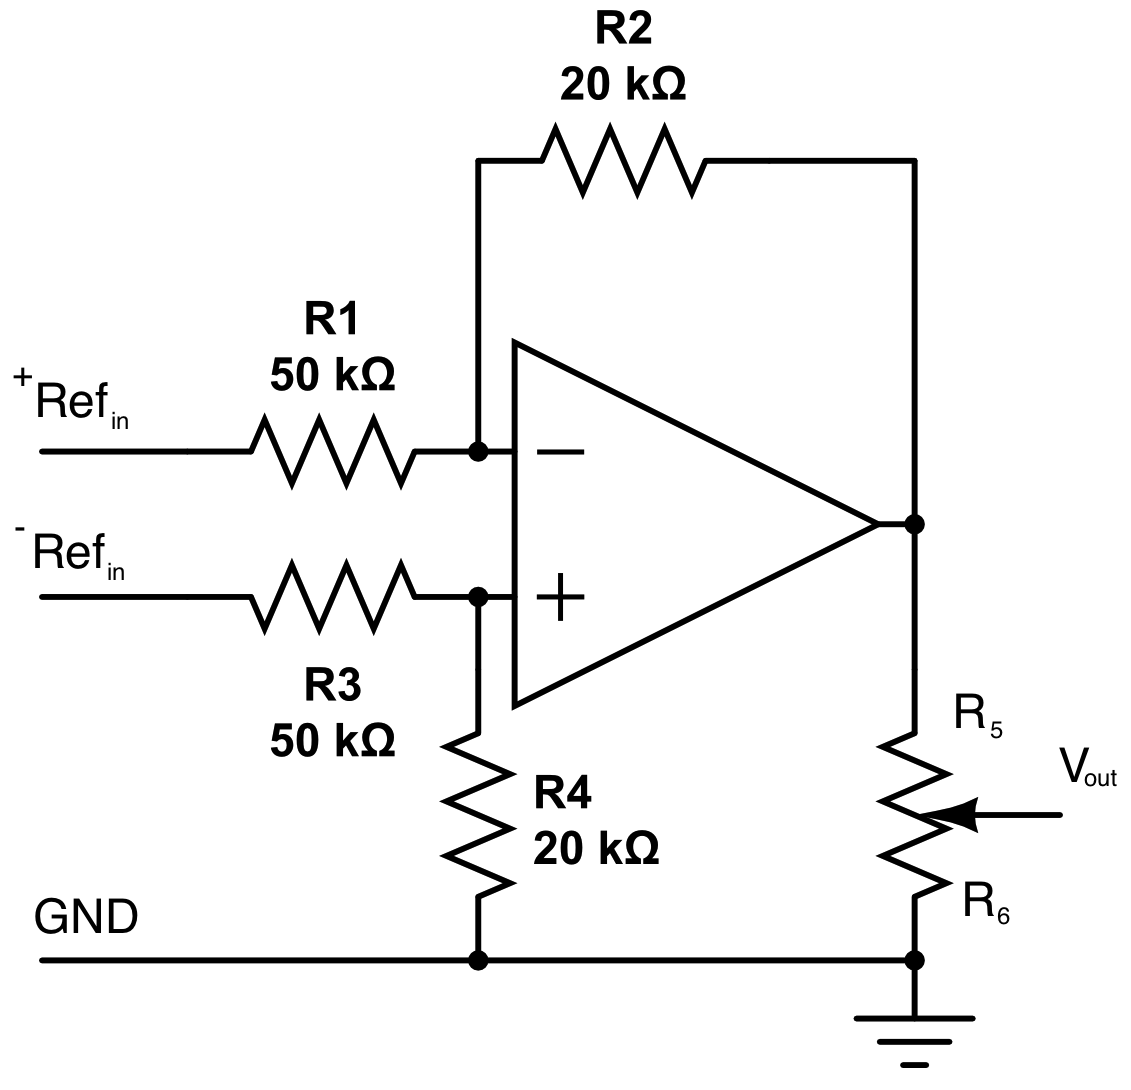
\includegraphics[width = 10cm]{q1a_u1.png}
\caption{Unit 1 within AMC servo-amplifier}
\label{q1_au1}
\end{center}
\end{figure}

\subsubsection*{U3}

U3 serves as an inverting amplifier which can be tuned by the potentiometer.

$$U3_{out} = - \left( \frac{R_3 + R_4}{R_4} \right) \left( \frac{R_2}{R_1} \right) Ref_{gain} $$
$$U3_{out} = - \left( \frac{R_3 + R_4}{R_4} \right) \left( \frac{10}{5} \right) Ref_{gain} $$

\begin{figure}[htb]
\begin{center}
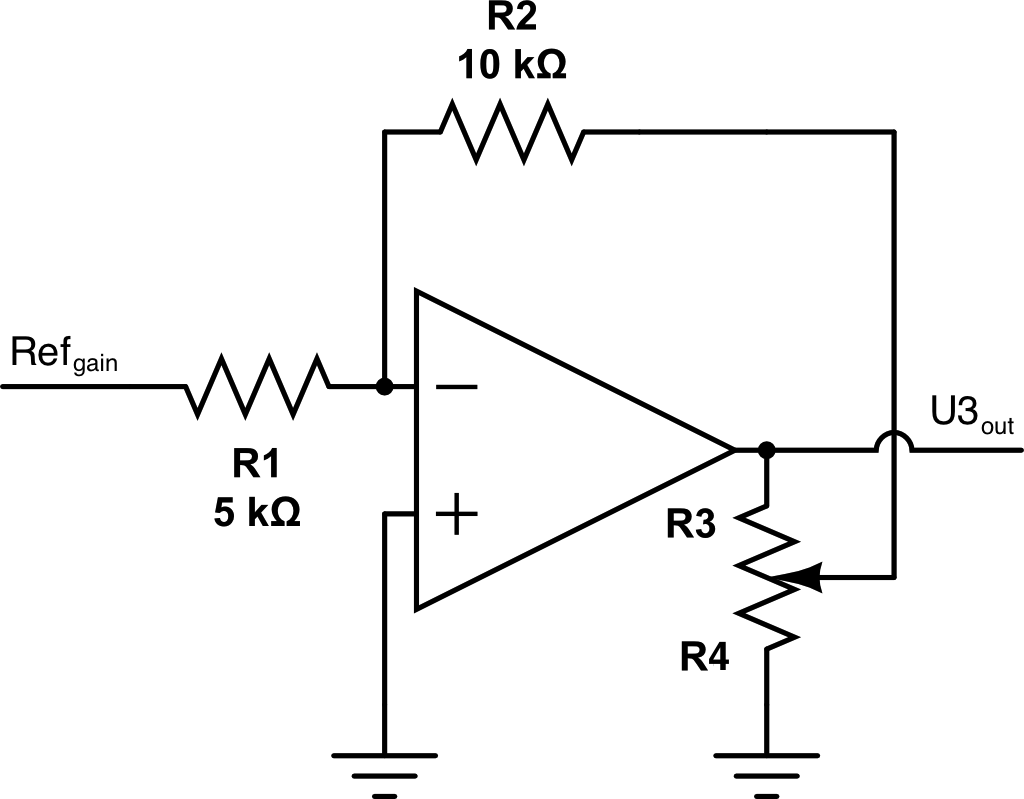
\includegraphics[width = 10cm]{q1a_u3.png}
\caption{Unit 3 within AMC servo-amplifier}
\label{q1_au3}
\end{center}
\end{figure}

\subsubsection*{U4}

U4 serves as an inverting integrator with a proportional gain when switch 3 is open, and a simple inverting amplifier with the switch closed.

$$U4_{out} = - \left( \frac{1}{R_1} \right) \left( R_2 + \frac{C_1}{s} \right) U3_{out} $$
$$U4_{out} = - \left( \frac{1}{500} \right) \left( 500 + \frac{0.01}{s} \right) U3_{out} $$

\begin{figure}[htb]
\begin{center}
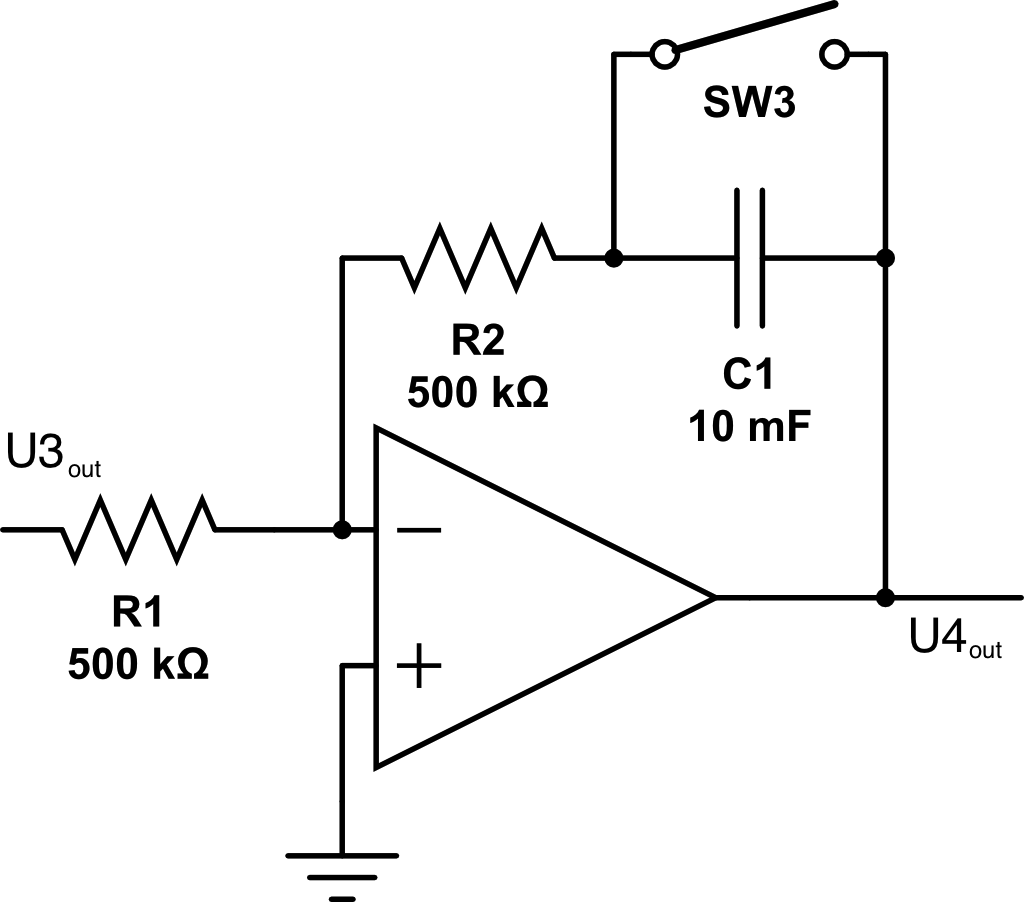
\includegraphics[width = 10cm]{q1a_u4.png}
\caption{Unit 4 within AMC servo-amplifier}
\label{q1_au4}
\end{center}
\end{figure}

\subsection*{b.}
Current Limiting Resistor.
For DC current, an inductor is effectively a short circuit.  We need a resistor to limit the maximum current that goes to ground.
\xxx{confirm with him that its a coil in series with resistor}

\subsection*{c.}
The motor datasheet specifies a max winding temerature of 155 $^\circ$C; this is the temperature at which the motor can become irreparably damaged. The datasheet also gives a thermal impedance of 11.2 $^\circ$C/W. Assuming a room temperature of 15 $^\circ$C, the motor's temperature can only increase by 130 $^\circ$C before overheating. With these values (and the motor's internal resistance of 1.85 $\Omega$) we can solve for the maximum continuous current:

$$130 = 11.2*i_{continuous}^2*1.85$$
$$i_{continuous} = 2.5048 \,A$$

With this current and the given motor constant we can then calculate the maximum continuous torque:

$$T_{m} = k_{t}*i_{continuous} = 3.11\e{-2}*2.5048 = 7.79\e{-2}\, Nm$$

This value is less than the torque value given in the datasheet, implying that our calculated current value is more conservative than the ratings in the datasheet. Based on the given rating for max continuous torque (8.1$\e{-2}$ Nm), the max continuous current would be 2.6045 A, but at that value the temperature rise would be 140.55 $^\circ$C above ambient. This means that at the max torque given by the datasheet, the motor would overheat unless the room temperature were below 14.45 $^\circ$C. 

The motor's datasheet lists a peak current rating of 13.0 A and a stall torque of 0.54 Nm. With this torque value and the given torque constant (4.24$\e{-2}$ Nm/A), the peak current should be:


$$i_{peak} = \frac{T_{stall}}{k_{t}} = \frac{0.54}{4.24\e{-2}} = 12.74 \,A$$

This is less than the given rating for peak current. Choosing this as our peak current limit, the power in the motor is:


$$P = i_{peak}^2 * R_{m} = 12.74^2 * 1.85 = 300.269 \,W$$

Because this is occuring at stall, there is no mechanical power output from the motor, and all of the power goes to heat. If the system were allowed to go to steady-state with no failures, this would lead to a temperature of:

$$Temp = P * R_{t} = 300.269 * 11.2 = 3363.0128  \,{^\circ}C\;(above \;ambient)$$ 

Clearly the system could not phyical reach this temperature without failing, but it illustrates the reason that peak current can only be sustained for short times. With the given thermal time constant (13.8 min), we can plot the temperature rise of the motor, as shown in figure \ref{temperature}, and estimate that it would overheat after approximately 32.4 seconds at peak current. 

\begin{figure}[htb]
\begin{center}
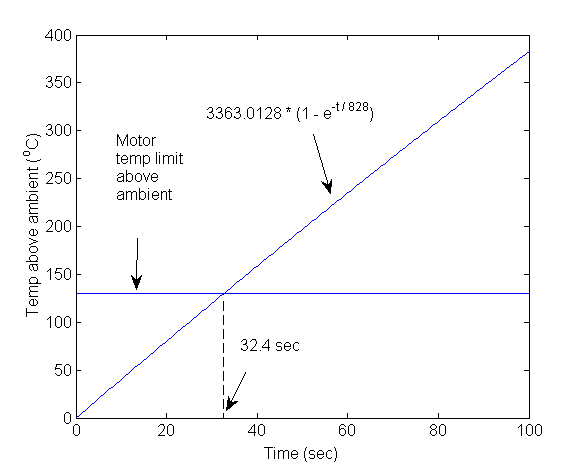
\includegraphics[width = 12cm]{temperature.png}
\caption{Motor temperature over time at peak current}
\label{temperature}
\end{center}
\end{figure}

\subsection*{d.}
The 12A8E servo amplifier is capable of outputting maximum continuous and peak currents of +-6A and +-12A, respecitvely (from the datasheet). However, the servo amplifier includes a potentiometer that can be used to reduce both the continuous and peak currents (while maintaining a 1:2 relationship between them). The lab instructions specify that the potentiometer should be adjusted so that the current limits will be +-3A and +-6A. Additionally, the continuous current limit can be further reduced (without affecting the peak current) by connecting a current limiting resistor between pins P1-10 and P1-2 on the servo-amp. That was not done in this lab. Assuming the adjustment on the current limiting potentiometer was done correctly, the servo-amp should be capable of sending +-3A continuously and +-6A intermittently to the motor. The continuous current limit from the servo-amp is greater than the continuous current rating of the motor, so we can't rely on the servo-amp to prevent the motor from drawing too much current.
\vspace{3 mm}

The datasheet for the servo-amp specifies a peak current of +-12 A for a maximum of 2 seconds. From information on the Advanced Motion Controls website, this can only be achieved if the current switches across its entire range (-12 A to +12 A, and vice-versa). Any change of smaller magnitude will not be maintained as long (i.e. switching from 0 A to +12 A will only be held for 1 second before the current begins falling). A primary concern with maintaining high currents is overheating, and the servo-amp has a much lower temperature limit than the motor (65 $^\circ$C vs 155 $^\circ$C). This is why the peak current can not be maintained for long, the maximum temperature would be exceeded very quickly and the servo-amp's internal safeties would shut it off. As an example, in the thermal model for the motor at peak current (which is lower than the 6 A rating of the servo-amp), 65 $^\circ$C was reached in only 9.8 seconds. Of course, the servo-amp has different thermal properties than the motor, so that specific value is not accurate. However, the basic idea is valid: the servo-amp is capable of passing a lot of current, and has a lower temperature limit than the motor, so there is a dange rof it overheating if high currents are maintained. Luckily, the servo-amp has built in safeties, such as a thermal shut-off.   

\subsection*{e.}
In the above sections, we showed that the motor has a continuous and peak current limits of 2.5 A and 12.74 A, and the servo-amp  has current limits of 3 A and 6 A, respecitvely. Within our LabView controller we chose to implement saturation limits of +-6 A so that we could take advantage of the peak current capability of the servo-amp and motor. We considered setting a saturation limit based on the motor's continuous current limit of 2.5 A, but felt that might have a negative effect on the transient response of the motor. Also, we knew that the servo-amp has built in mechanisms to prevent the current from remaining at the peak value - it automatically lowers it after at most two seconds. Additionally, as we were tuning our LabView controller, we monitored a waveform graph of the attempted output of the contoller. This allowed us to adjust our gain values not just for system stability, but also to keep the attempted output within safe limits. Given more resources, we could have implemented more safety measures. For example, we could implement a slow-blow fuse rated a little under the continuous current limit of the motor. This would protect the system from high currents for prolonged times, but still allow for short bursts of higher current during transient conditions.

\section*{2.}

\subsection*{a.}

Using expressions for the back-emf of the motor with a simple model of the motor as a resistance in series with an inductance we can model the electrical characteristics of the motor.  We can combine this with a simple lumped parameter model of physical dynamics of the motor to derive an overall transfer function.  
$$V_{s} - e = iR + L\left(\frac{di}{dt}\right) $$
$$ e = K_{b} \dot{\theta} $$

$$ \Sigma_{\tau} = \tau_{motor} - \tau_{damping} + \tau_{coulomb} = J \ddot{\theta}$$
$$ \tau_{motor} = K_{T}i \hspace{1cm} \tau_{damping} = b \dot{\theta}$$

\[
  \tau_{coulomb} = \left\{
  \begin{array}{c l}
	 - \tau_{motor} & \quad \text{if } \dot{\theta} = 0 \text{ and } |\tau_{motor}| < \tau_{friction} \\
	- sgn(\tau_{motor}) \cdot \tau_{friction} & \quad \text{if } \dot{\theta} = 0 \text{ and } |\tau_{motor}| > \tau_{friction} \\
	- sgn(\dot{\theta}) \cdot \tau_{friction} & \quad \text{if } \dot{\theta} \neq 0 \\
%    	- \mu_{kinetic}N & \quad \text{if } \dot{\theta} > 0 \\
%    	+ \mu_{kinetic}N & \quad \text{if } \dot{\theta} < 0 \\
%	- \mu_{static}N & \quad \text{if } \dot{\theta} = 0 \text{ and } \tau_{motor} > \mu_{static}N \\
%	- \tau_{motor} & \quad \text{if } \dot{\theta} = 0 \text{ and } 0 <= \tau_{motor} <= \mu_{static}N \\
%	+ \mu_{static}N & \quad \text{if } \dot{\theta} = 0 \text{ and } \tau_{motor} < -\mu_{static}N \\
%	+ \tau_{motor} & \quad \text{if } \dot{\theta} = 0 \text{ and } 0 >=\tau_{motor} >= -\mu_{static}N \\
  \end{array} \right.
\]

Where: $K_{t}$ is the motor torque constant; $J$ is the rotor inertia; $b$ is the viscous damping on the rotor; $K_{b}$ is the back-emf constant of the motor; $R$ is the equivalent resistance of the motor; $L$ is the effective motor inductance; $i$ is the current flowing through the motor; and $\tau_{coulomb}$ is the force of coulomb friction on the rotor. \\

Neglecting coulomb friction:

$$ V_{s}(s) - s \, K_{b} \, \theta (s) = I(s) (R+sL) \hspace{1cm} \text{and} \hspace{1cm} K_{t} \, I(s) = \theta(s)(Js^2+bs) $$
$$ \frac{\theta(s)}{V(s)} = \frac{K_T}{s\left[ (Js + b)(Ls + R)+K_bK_T \right]} $$

The transfer function relating voltage and position is not particularly convenient but we can obtain a transfer function easily in terms of $I(s)$.

$$ K_{t} \, I(s) = \theta(s)(Js^2+bs) $$
$$ \frac{\theta(s)}{I(s)} = \frac{K_T}{(Js + b)s} $$

This model relating angular position, $\theta(t)$ with motor current $i(t)$ requires the moment of inertia of the rotor, $J$, the viscous damping coefficient, $b$, and the torque constant $K_T$.  Note that coulomb friction has been neglected. \\

The driver gives us current control as long as we are opperating away from the maximum speed of the motor.  At maximum speed, the current required by the motor should drop to some steady state value required to overcome losses within the motor.

\xxx{may need to redo picture a bit to agree with terminology in equation}
\begin{figure}[htb]
\begin{center}
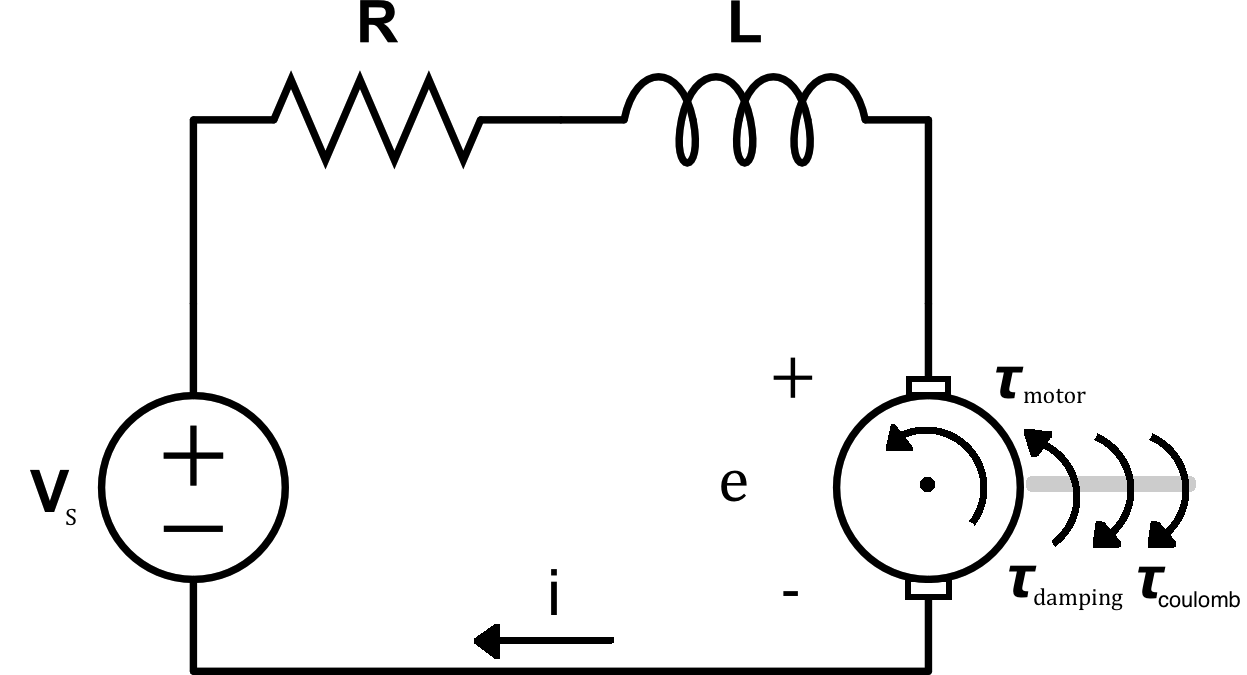
\includegraphics[width = 13cm]{dcmotor.png}
\caption{DC motor model}
\label{q2_a1}
\end{center}
\end{figure}

\subsection*{b.}

The torque of friction and the viscous damping can be jointly  derived in an experiment where for a given constant input voltage to the driver, $V_{driver}$, we read off the angular velocity.  At a constant velocity the following equation holds giving a relationship between $\tau_{motor}$, $b$, and $\tau_{coulomb}$.

$$\Sigma_{\tau} =  \tau_{motor} - b\dot{\theta} + \tau_{coulomb} = J \ddot{\theta} \hspace{1cm} \ddot{\theta} = 0 $$
$$ \tau_{motor} = K_{T}I_{m} = b\dot{\theta}_{ss} - \tau_{coulomb}$$

Assuming that we have the motor torque constant $K_{t}$, we can write an equation that relates steady state angular velocity $\theta_{steady state}$ to motor current which is known to be directly proportional to $V_{driver}$ for suitably small values of $V_{driver}$.

$$ V_{driver} = I_{m} \hspace{1cm} V_{driver} = \left( \frac{b}{K_T} \right) \dot{\theta}_{ss} - \frac{\tau_{coulomb}}{K_{T}} $$

From our plot in figure \ref{q2_b4} we can obtain $\left( \sfrac{b}{K_t} \right)$ as the slope of each of the linear segments and $\sfrac{\tau_{coulomb}}{K_{T}}$ as the y intercepts shown in table \ref{q2_b5}.  We can separately determine the force of static friction $\tau_{static \, coulomb}$ by measuring the smallest input voltage to the driver, and from this how much torque, is required to start the motor from rest.

$$ \Sigma_{\tau} =  \tau_{motor} - b\dot{\theta} + \tau_{coulomb} = J \ddot{\theta} \hspace{1cm} \dot{\theta} = \ddot{\theta} = 0 $$
$$ V_{driver} = - \frac{\tau_{coulomb}}{K_{T}} $$

\begin{figure}[htb]
\begin{center}
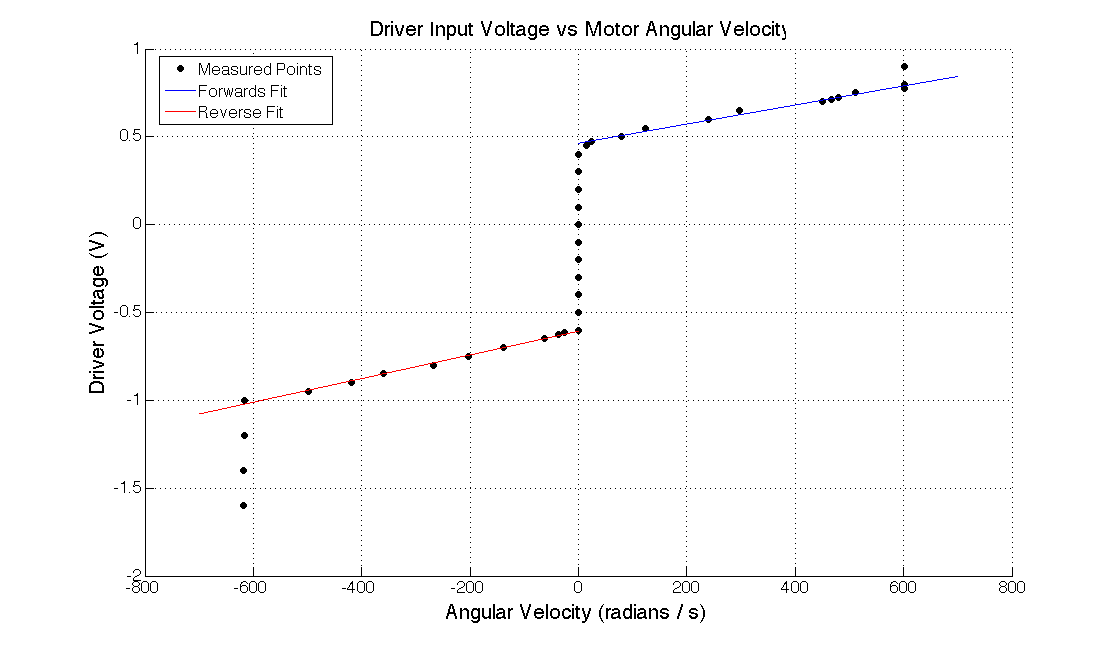
\includegraphics[width = 16cm]{SpeedCurrentCurve.png}
\caption{Relationship between angular velocity and steady state voltage applied to motor driver}
\label{q2_b4}
\end{center}
\end{figure}

\begin{table}[htb]
\begin{center}
    \begin{tabular}{|c|c|c|}
        \hline
        ~        & Slope $\left( \frac{V * s}{rad} \right) $ & y-intercept $ \left( V \right) $ \\ \hline
        Forwards & 5.4289e-04                                & 0.46374                          \\ 
        Reverse  & 6.72805e-04                               & -0.60717                         \\
        \hline
    \end{tabular}
\end{center}
\caption{Extracted slopes and y-intercepts from current speed curve}
\label{q2_b5}
\end{table}

To compute the torque constant, $K_{T}$ we can first compute the back-emf constant, $K_b$, which we know to be numerically equal to $K_T$ in SI units.  To calculate $K_b$ we can measure the internal resistance of the motor, R, using an ohm-meter.  Then running the system at a constant current, we can measure the source voltage, $V_{s}$ that the driver outputs to maintain that current  to obtain e. We can use the encoder to measure the angular velocity and use that value with e to solve for $K_b$

$$ \Sigma_{V} = V_{s} + V_{R} + V_{L} e = V_{s} + IR + e = 0 $$
$$ K_b = \frac{e}{\dot{\theta}} $$

%To determine the torque constant, we can place the motor on its side, pin a pulley to the shaft and attach a known mass to the pulley.  This exerts a known torque on the shaft, and we can simply adjust motor current until it balances out the torque.   
%
%$$ \Sigma_{tau} = \tau_{motor} - b\dot{\theta} + \tau_{coulomb} - \tau_{mass}= J \ddot{\theta} \hspace{1cm} \dot{\theta} = \ddot{\theta} = 0  $$
%$$ \tau_{motor} = - \tau_{coulomb} + \tau_{mass} \approx \tau_{mass} $$
%
%$$ K_T \approx \frac{\tau_{mass}}{i_{equilibrium}} = \frac{mg(r_{pulley})}{i_{equilibrium}} $$

We can experimentally determine the viscous damping term, $b$ by applying a known torque to the motor.  Once the angular velocity has reached steady state, $b$ can be read off directly.  The driver in current mode delivers a known current, which using the torque constant determined above yields the torque.  

$$ \Sigma_{tau} = \tau_{motor} - b\dot{\theta} + \tau_{coulomb} = J \ddot{\theta} \hspace{1cm} \ddot{\theta} = 0 $$
$$ b = \frac{\tau_{motor} + \tau_{coulomb}}{\dot{\theta}} \approx \frac{\tau_{motor}}{\dot{\theta}}$$

We can determine the moment of inertia of the rotor, $J$ by starting from rest and sending the motor a known torque while recording the position as a function of time stopping when the system has reached a constant velocity.  Then by computing the $1^{st}$ and $2^{nd}$ order derivatives at each time step we can assemble a linear system to allow us to jointly solve for $J$, $b$, and $\tau_{coulomb}$.

$$ A_{t} = \left[ \begin{array}{c c c} \ddot{\theta_{t}} & \dot{\theta_{t}} & -1 \end{array} \right]  \hspace{1cm} 
x = \left[ \begin{array}{c} J \\ b \\ \tau_{coulomb} \end{array} \right] \hspace{1cm} z_{t} = \tau_{motor} $$
$$ Ax = z $$

Rather than attempt the method above, we instead used MATLAB's numerical differential equation solving to simulate the trajectory of the system as a function of time, driver current, $I_t$ and our unknown system parameters $J$, $b$, $K_t$, and $\tau_{coulomb}$.  By then
comparing the predicted angular positions with the measured angular positions over time, we can construct a non-linear regression to estimate the unknown parameters.  We collected a data set where the driver was given a sinusoidal voltage, and we assume that motor current, $I_m$, is identical to this driver voltage and recorded the motor motion that this input caused. \\

Table \ref{q2_b1} below shows the parameters for our equation of motion obtained from the data sheet.  The results, in figure \ref{q2_b2} shows the estimated trajectory using these parameter values.  It is very clear that these parameter values are quite far off.  Attempting to perform nonlinear optimization on our model parameters proved to be very difficult yielding fits similar to the results shown in figure \ref{q2_b6}.  It is clear that although these  results are significantly improved over the original values, but there is still room for improvement.  However, improvement from this minima is not possible strictly using the method noted above, so we resorted to parameter sweeping to to identify more appropriate values.  Figure \ref{q2_b7} shows one of the best results discovered by this parameter sweep.  In this case the error has been reduced, but the fit still appear inappropriate.  \\

\begin{table}[htb]
\begin{center}
    \begin{tabular}{|c|c|}
        \hline
        ~                                                      & Data Sheet Parameters        \\ \hline
        $J \hspace{0.1cm} \left( \frac{N\cdot s^2}{m} \right)$     & $8.5 \cdot 10^{-6} $               \\ 
        $b \hspace{0.1cm} \left( N \cdot s \right) $               & $3.7\cdot 10^{-6} $                 \\ 
        $\tau_{coulomb} \hspace{0.1cm} \left( N \cdot m \right)$           & $\frac{5.6 \cdot 10^{-3}}{2} $  \\ 
        $K_{T} \hspace{0.1cm} \left( \frac{N\cdot m}{A} \right) $ & $4.24 \cdot 10^{-2}$             \\
        \hline
    \end{tabular}
\caption{Comparison of model parameter values obtained from the data sheet to fit values.}
\label{q2_b1}
\end{center}
\end{table}

\begin{figure}[htb]
\begin{center}
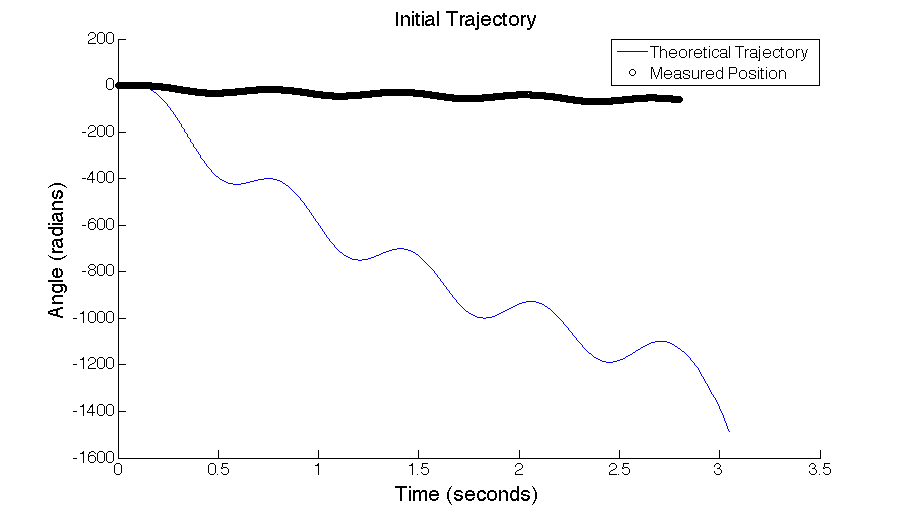
\includegraphics[width = 14cm]{initialModel.png}
\caption{Predicted behavior vs Actual behavior using initial parameter values.}
\label{q2_b2}
\end{center}
\end{figure}

\begin{figure}[htb]
\begin{center}
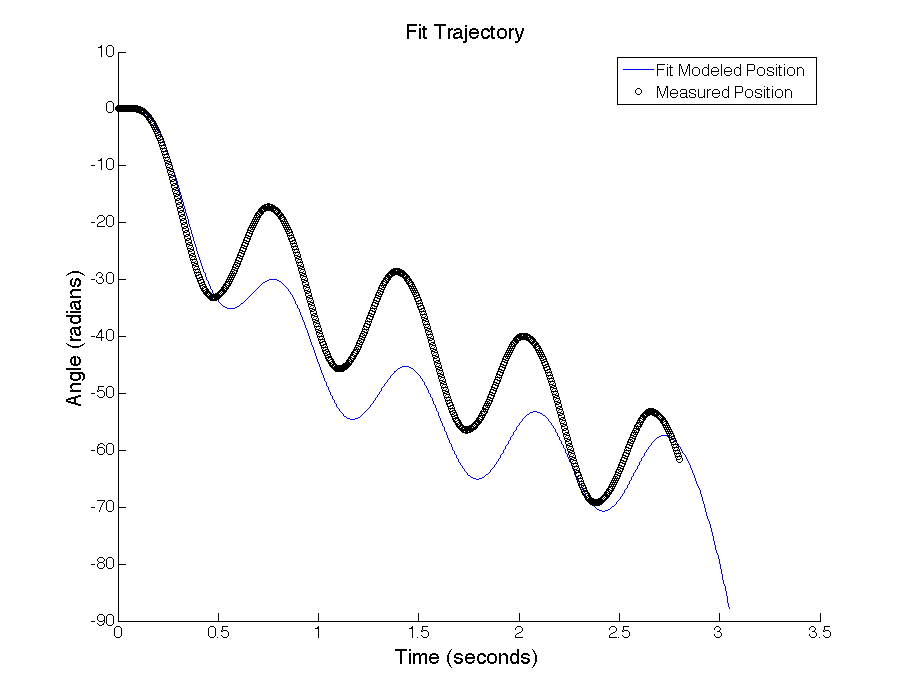
\includegraphics[width = 14cm]{fitModel.png}
\caption{Example of local minimum in error.  $J = 0.001 \, B = 0.001 \, F_{f} = 0.1192 \, K_{t} = 0.0467 $}
\label{q2_b6}
\end{center}
\end{figure}

\begin{figure}[htb]
\begin{center}
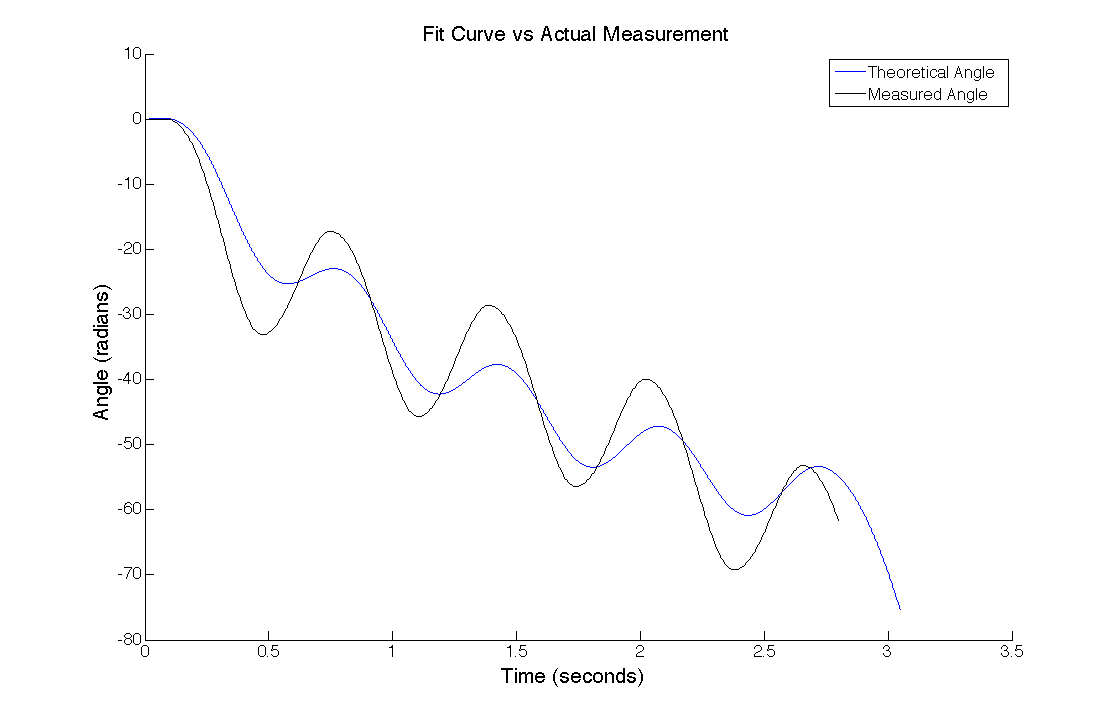
\includegraphics[width = 14cm]{2ndexamplefit.png}
\caption{Improved Fit $J = 6.06724 \cdot 10^{-5} \, B = 4.05562 \cdot 10^{-5} \, F_{f} = 0.0145312 \, K_{t} = 0.019020 $}
\label{q2_b7}
\end{center}
\end{figure}

Manual parameter guessing revealed that it was not possible to obtain the measured curve using the model, repeated below. 
$$ \Sigma_{tau} = K_{T}I_{m} - b\dot{\theta} + \tau_{coulomb} = J \ddot{\theta} $$

Clearly there were some effects that this model neglected.  Our previous experiment to attempt to determine $b$ and $\tau_{coulomb}$ showed that these parameters are likely not the same in each direction, so we augmented the model to allow $b$ and $\tau_{coulomb}$ to take on different values in the forwards direction and reverse directions yielding the following model:

$$ \Sigma_{tau} = \tau_{motor} - b\dot{\theta} + \tau_{coulomb} = J \ddot{\theta} $$

\[
  \tau_{coulomb} = \left\{
  \begin{array}{l l}
    	- \tau_{forwards} & \quad \text{if } \dot{\theta} > 0 \\
    	+ \tau_{reverse} & \quad \text{if } \dot{\theta} < 0 \\
	- \tau_{forwards} & \quad \text{if } \dot{\theta} = 0 \text{ and } \tau_{motor} > \tau_{forwards} \\
	- \tau_{motor} & \quad \text{if } \dot{\theta} = 0 \text{ and } 0 <= \tau_{motor} <= \tau_{forwards} \\
	+ \tau_{reverse} & \quad \text{if } \dot{\theta} = 0 \text{ and } \tau_{motor} < -\tau_{reverse} \\
	+ \tau_{motor} & \quad \text{if } \dot{\theta} = 0 \text{ and } 0 >=\tau_{motor} >= -\tau_{reverse}\\
  \end{array} \right.
\]

\[
b = \left\{
\begin{array}{l l}
b_{forwards} & \quad \text{if } \dot{\theta} > 0 \\
b_{reverse} & \quad  \text{if } \dot{\theta} < 0 \\
\end{array} \right.
\]

With this improved model and some intelligent guessing for new parameter values, we arrived at an excellent fit shown in figure \ref{q2_b3}.
The most notable feature of these values is the large difference between the torque of friction in the forwards and reverse directions.  

\begin{table}[htb]
\begin{center}
    \begin{tabular}{|c|c|c|}
        \hline
        ~                 & Data-Sheet Values    & Fit Values              \\ \hline
        $J \hspace{0.1cm} \left( \frac{N \cdot s^2}{m} \right)$               & $8.5 \cdot 10^{-6} $     & $3.50514 \cdot 10^{-5}$ \\ 
        $K_{t} \hspace{0.1cm} \left( \frac{N\cdot m}{A} \right)$           & $0.0424$             & $0.0314499$             \\ 
        $b_{forwards} \hspace{0.1cm} \left( N \cdot s \right)$    & $3.7 \cdot 10^{-6} $ & $1.08586 \cdot 10^{-5}$ \\ 
        $b_{reverse} \hspace{0.1cm} \left( N \cdot s \right)$     & $3.7 \cdot 10^{-6} $ & $2.49301 \cdot 10^{-5}$ \\ 
        $\tau_{forwards} \hspace{0.1cm} \left( N \cdot m \right)$ & $5.6 \cdot 10^{-3}$  & $0.0224389$             \\ 
        $\tau_{reverse} \hspace{0.1cm} \left( N \cdot m \right)$   & $5.6 \cdot 10^{-3}$  & $0.0143096$             \\
        \hline
    \end{tabular}
\caption{Final Parameter Values vs Original Data Sheet Values}
\label{q2_b8}
\end{center}
\end{table}

Table \ref{q2_b1} below shows our final fit values alongside the original values obtained from the data sheet.  This large difference in values is clearly illustrated by the large difference in behavior between the actual system and our model using the values obtained from the data sheet shown in figure \ref{q2_b2}.  The results of fitting are shown in figure \ref{q2_b3}. We can also compare these fit values with values obtained from our earlier experiment.  We can notice that our terms are in the same order of magnitude, however it seems as if this experiment did not accurately estimate the force of friction as the relative values seem to be flipped between the two experiments. \\

\begin{table}[htb]
\begin{center}
    \begin{tabular}{|c|c|l|}
        \hline
        ~                 & Predicted Value          & Fit Value               \\ \hline
        $B_{forwards}$    & $1.707338 \cdot 10^{-5}$ & $1.08586 \cdot 10^{-5}$ \\ 
        $B_{reverse}$     & $2.11611 \cdot 10^{-5}$  & $2.49301 \cdot 10^{-5}$ \\ 
        $\tau_{forwards}$ & $0.0145846$              & $0.0224389$             \\ 
        $\tau_{reverse}$  & $0.0190954$              & $0.0143096$             \\
        \hline
    \end{tabular}
\caption{Damping and friction torques calculated from earlier experiment vs fit values}
\label{q2_b9}
\end{center}
\end{table}

\begin{figure}[htb]
\begin{center}
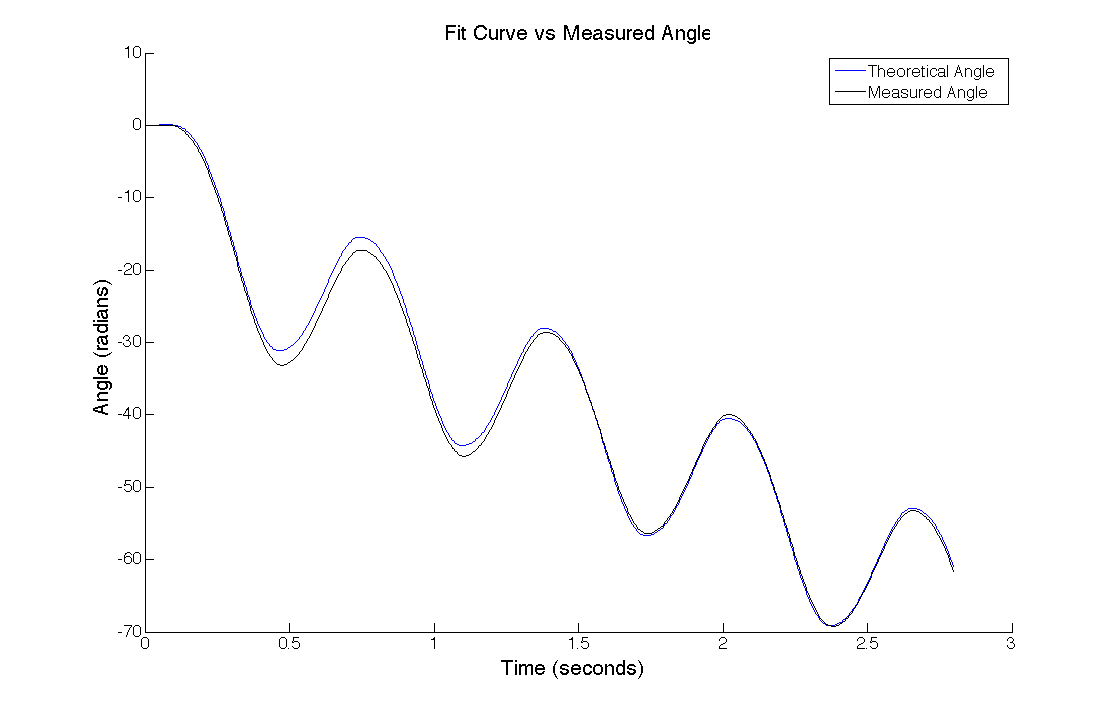
\includegraphics[width = 14cm]{awesomefitFiner.png}
\caption{Predicted behavior vs Actual behavior using fit parameter values and enhanced modeling}
\label{q2_b3}
\end{center}
\end{figure}

\section*{3.}
\subsection*{a.}

\subsection*{b.}

\subsection*{c.}

\subsection*{d.}

\subsection*{e.}

\subsection*{f.}

\section*{4.}

\subsection*{a.}
When we implemented the controller and values from our simulation in part 3, we were unable to achieve stable output in the physical system. Therefore, we kept the same general approach - a velocity controller nested within a position controller with feed forward - but we re-tuned the system with different gain values. Because we have a velocity controller inside of our position controller, we first tuned the velocity control on its own (see section 6). Once it was working, we then implemented it in the inner loop of our position controller and tuned the position control gains. In the end we were not able to meet all of the control goals with one controller. We designed one controller with good step response and noise attenuation, and then modified the gain values to improve the frequency response separately. The results for the step response and noise attenuation are given below.  

\begin{table}[htb]
\begin{center}
    \begin{tabular}{|c|c|c|c|c|c|}
        \hline
        Gains & P   & I & D   & Feed Forward   & Filter $\tau$   \\ \hline
        Position Loop            & 0.1 & 20  & 0 & 1 & 6.5797    \\ 
        Velocity Loop       & 22.5   & 22.5    & 1.125   & -  & 6.5797  \\ 
       \hline
    \end{tabular}
\end{center}
\caption{Values of position controller with nested velocity controller for step response and noise attenuation}
\label{positionGains}
\end{table}

Figure \ref{PosStepPi} shows the system's response to a position step input of 2$\pi$ radians, and figure \ref{PosStepError} shows a zoomed in view after it had settled. The error here is approximately 0.11\%, which greatly exceeds the goal of 2\% error.
\xxx{Compare to simulation results}

\begin{figure}[htb]
\begin{center}
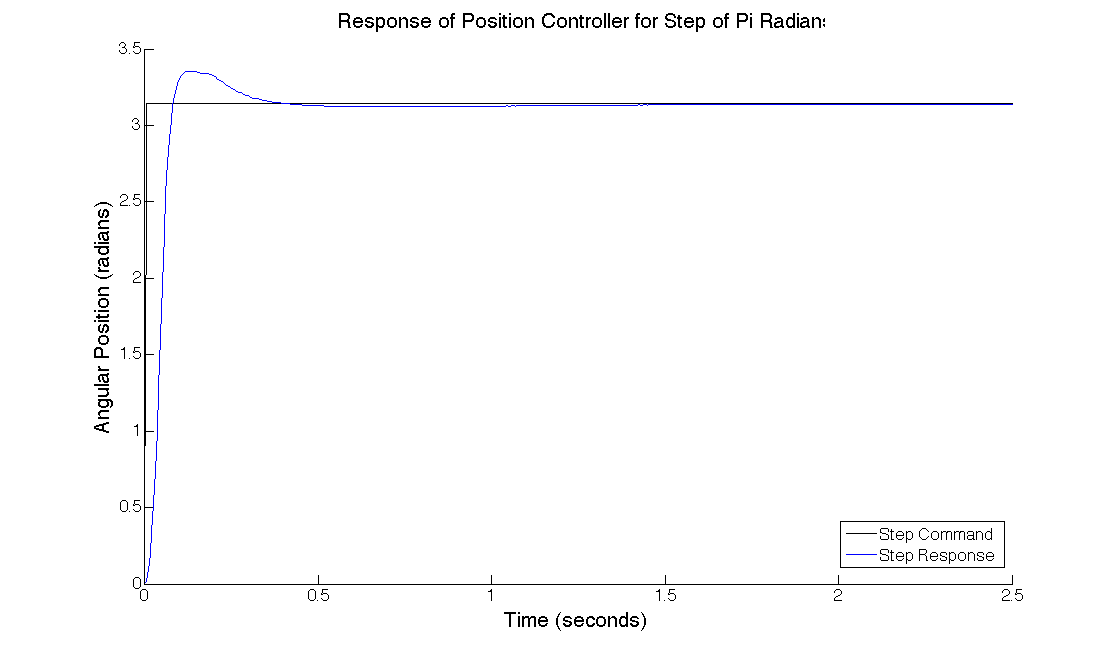
\includegraphics[width = 14cm]{posstep_1pi.png}
\caption{Step response of position controller}
\label{PosStepPi}
\end{center}
\end{figure}

\begin{figure}[htb]
\begin{center}
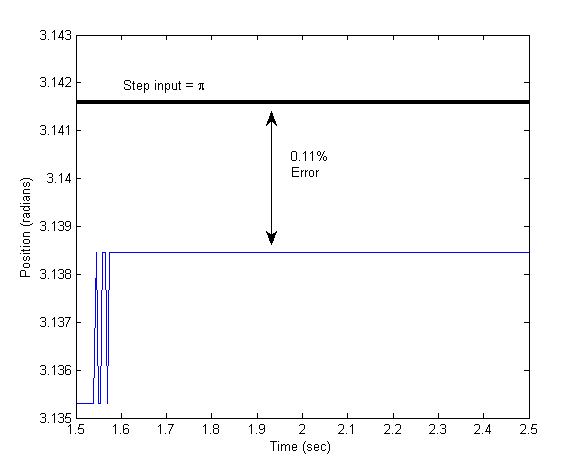
\includegraphics[width = 12cm]{positionStepError.png}
\caption{Steady state error for position step input of $\pi$}
\label{PosStepError}
\end{center}
\end{figure}

Figure \ref{PosNoise} shows the noise attenuation during a step input of pi radians. To simulate the noise within LabView, we added a 60 Hz sine signal with an amplitude of 1 to the output of the DAQ assistant. Figure \ref{PosNoiseZoom} shows a zoomed in view after the step has taken place. For the step response with no noise, our steady state error was approximately 0.003, and with the noise the highest error is 0.060. Given that we were inputting a noise amplitude of one and the error only increased by 0.057, we have attenuated the noise by approximately 17.54 times. This exceeds the goal of a ten times reduction.
\xxx{Compare to simulation results}

\begin{figure}[htb]
\begin{center}
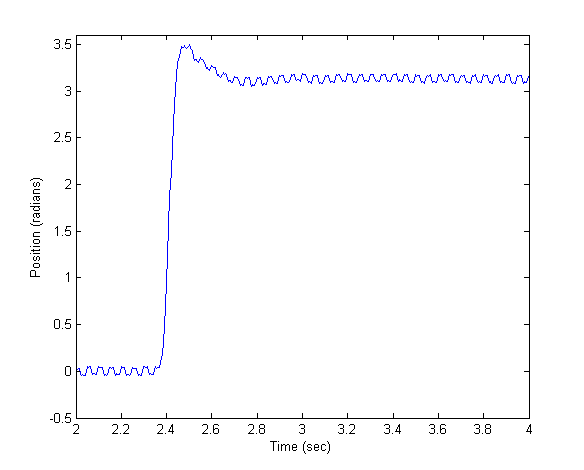
\includegraphics[width = 12cm]{PosNoise.png}
\caption{Step response for input of $\pi$ with a 60 Hz noise signal (amplitude = 1)}
\label{PosNoise}
\end{center}
\end{figure}

\begin{figure}[htb]
\begin{center}
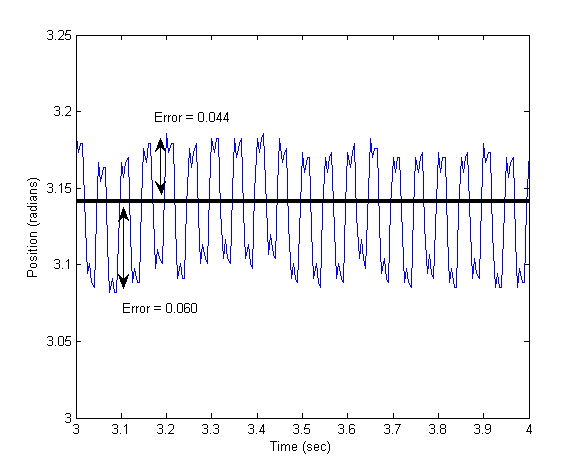
\includegraphics[width = 12cm]{PosNoiseZoom.png}
\caption{Steady state step response for input of $\pi$ with a 60 Hz noise signal (amplitude = 1)}
\label{PosNoiseZoom}
\end{center}
\end{figure}

The position controller we were using for the step response and noise attenuation did not not perform well with sinusoidal inputs, therefore we modified to gains while keeping the overall architecture the same. The relevant values are given in the following table, and the following figures show the response at various frequencies with an amplitude of $\pi$. Figure \ref{PosFreqError} shows the error as a function of input frequency. During our tests the position output remained stable up to 5 Hz, but the output amplitude error exceeded 5\% just beyond 4 Hz. This does not meet the goal of less than 5\% error up to 5 Hz.
\xxx{Compare to simulation}

\begin{table}[htb]
\begin{center}
    \begin{tabular}{|c|c|c|c|c|c|}
        \hline
        Gains & P   & I & D   & Feed Forward   & Filter $\tau$   \\ \hline
        Position Loop            & 0 & 20  & 0 & 1 & 6.5797    \\ 
        Velocity Loop       & 3   & 7    & 0.4   & -  & 6.5797  \\ 
       \hline
    \end{tabular}
\end{center}
\caption{Values of position controller with nested velocity controller for frequency response}
\label{positionGains}
\end{table}

\begin{figure}[htb]
\begin{center}
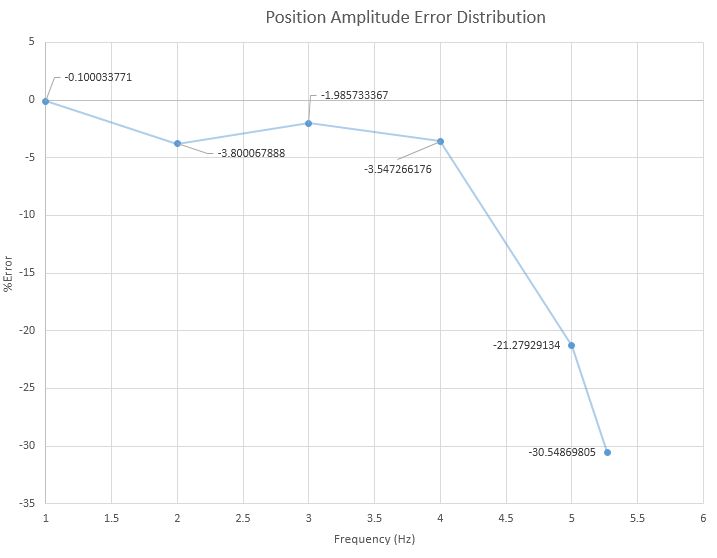
\includegraphics[width = 14cm]{PositionControl_Error.png}
\caption{Position error vs. frequency for an input amplitude of $\pi$ radians}
\label{PosFreqError}
\end{center}
\end{figure}

To determine the closed-loop bandwidth of the system, we slowly increased the frequency of the input signal until the output amplitude just crossed -3 dB (for a input of $\pi$ this corresponded to an output of 2.22). We found that the bandwidth of our position control system was 5.27 Hz, as shown in figure \ref{PosBandwidth}.

\begin{figure}[htb]
\begin{center}
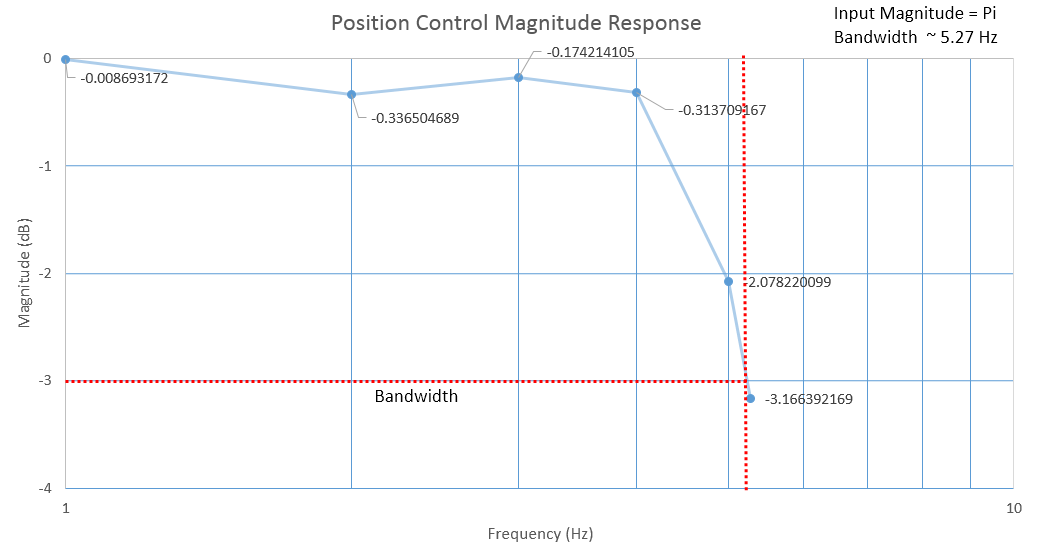
\includegraphics[width = 14cm]{PositionControl_Magnitude.png}
\caption{Output magnitude vs. frequency used to determine bandwidth}
\label{PosBandwidth}
\end{center}
\end{figure}

Even though we included many nonlinear factors in our simulation, we still faced a lot of trouble meeting all of the performance specifications, particularly trying to do so with just one controller. In general, we found that when we adjusted gains to meet the step requirement, the frequency response usually got worse, and vice-versa. It's possible that some of the values used in our simulation are incorrect (even after testing and regression), or that there are other factors we did not account for, such as the dynamics of the servo-amp. In th end we were able to meet the steady state error for step input and noise attenuation requirements, and were very close to the frequency response requirement.

\section*{5.}

\subsection*{a. Coulomb Friction}
The bearings in the motor are the primary source of coulomb friction in the motor encoder system. This could be especially true in the current configuration of the motor because Pittman's website only specifies that they use ball or sleeve bearings in their products. If these are only radial bearings with no thrust capability, then the motor's performance could be affected by the vertical mounting we are using. Additionally, there is friction between the brushes and commutator. In section 2b we discussed and carried out experiments and modeling to determine the friction value.   

\vspace{3 mm}
Setting aside the earlier parameter identification, there are some simple experiments that could be run to estimate the friction in the system. If we assume that the torque constant given in the data-sheet is correct and that the gain of the servo-amp is exact and known, then for a given command voltage, the motor should be capable of a specific torque output. By slowly increasing the voltage from zero until the motor just begins to turn. From this, the torque caused by static friction would be equal to the product of the torque constant and the input voltage (because there is a 1:1 relationship between command voltage and applied current). 

\vspace{3 mm}
A similar method could be used to determine sliding friction. By applying a constant voltage to the system, the motor would come to a steady-state velocity. If we the coefficient of damping is known, then the torque caused by sliding friction is equal to the motor torque ($K_{t}$ * $V_{command}$) minus the torque from damping (the product of the damping coefficient and velocity). This was carried out in part 2b.

\vspace{3 mm}
Friction was included in our Simulink model from the beginning of our modeling, as presented in part 3. At the beginning of our tests we used approximations based on the data-sheet values, but as we performed more regression analysis, we obtained new values that should be closer to the true values of the physical system. 

\subsection*{b. Saturation}

Position Saturation

\xxx{comment on actuation saturation}

\begin{table}[htb]
\begin{center}
    \begin{tabular}{|c|c|c|c|c|c|}
        \hline
        Step Input Amplitude (Radians) & $1\pi$   & $1.5 \pi$ & $2\pi$   & $3\pi$   & $4\pi$   \\ \hline
        Rise Time (seconds)            & 0.0700002 & 0.0800000   & 0.0850000 & 0.110000 & 0.125    \\ 
        Settling Time (seconds)        & 0.290000   & 0.320000    & 0.28000   & 0.54500  & 1.45500  \\ 
        Percent Overshoot (\%)          & 6.79997   & 16.8000     & 31.8500   & 65.0331  & 91.0003  \\ 
        Steady State Error (\%)         & 0.100034  & 0.594022    & 0.150008  & 0.13335  & 0.399713 \\
        \hline
    \end{tabular}
\end{center}
\caption{Step Response for a variety of input positions.  Where rise time is defined as reaching 90\% of the final value while settling time is the time after which the function remains within 2\% of its final value}
\label{q5_b6}
\end{table}

\begin{figure}
\begin{center}
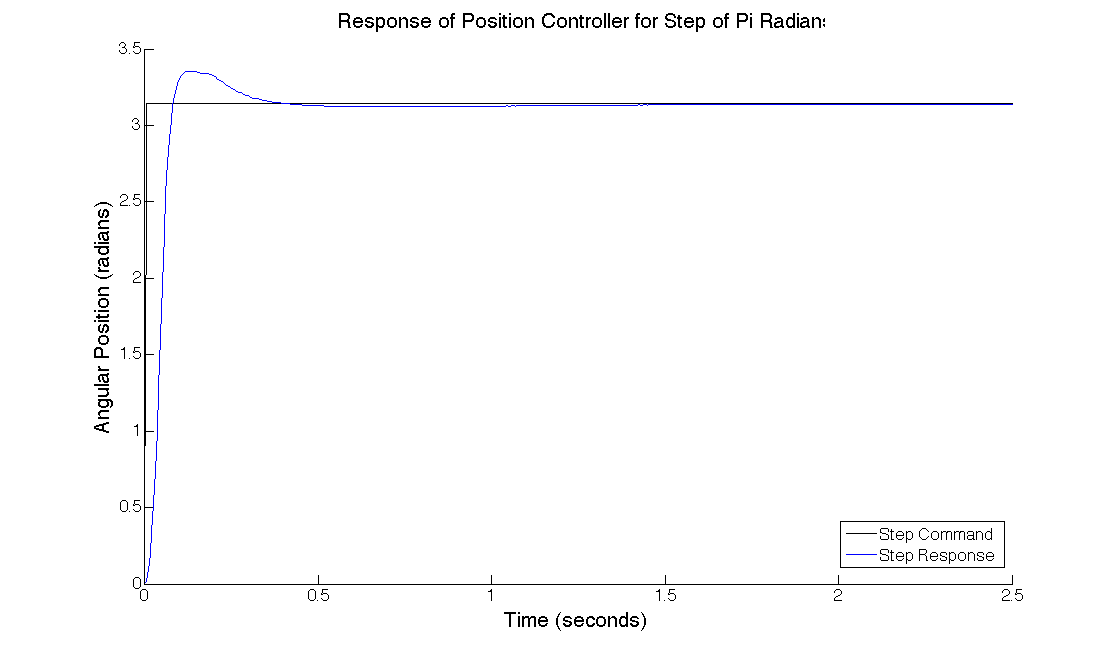
\includegraphics[width = 14cm]{posstep_1pi.png}
\caption{Step response of position controller}
\label{q5_b1}
\end{center}
\end{figure}

\begin{figure}
\begin{center}
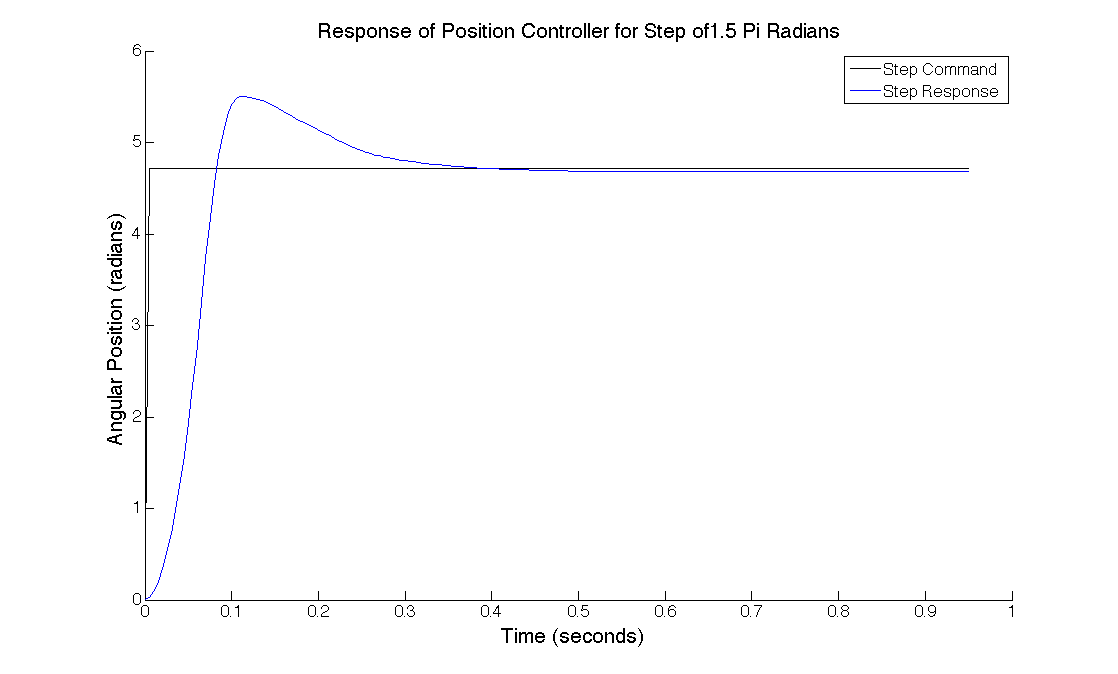
\includegraphics[width = 14cm]{posstep_15pi.png}
\caption{Step response of position controller}
\label{q5_b2}
\end{center}
\end{figure}

\begin{figure}
\begin{center}
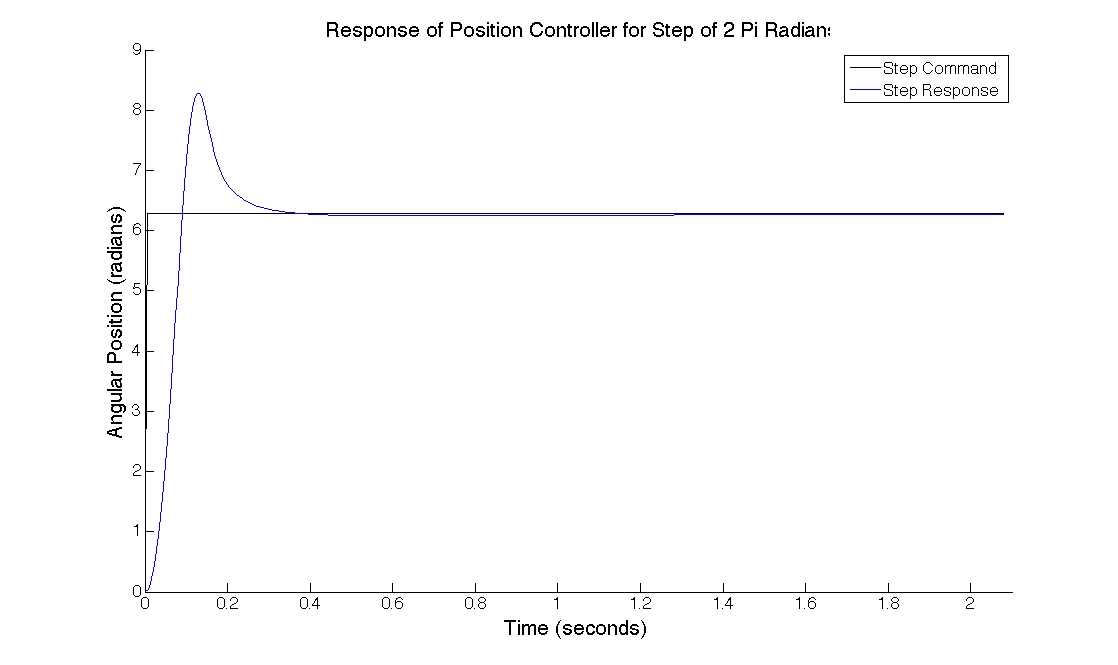
\includegraphics[width = 14cm]{posstep_2pi.png}
\caption{Step response of position controller}
\label{q5_b3}
\end{center}
\end{figure}

\begin{figure}
\begin{center}
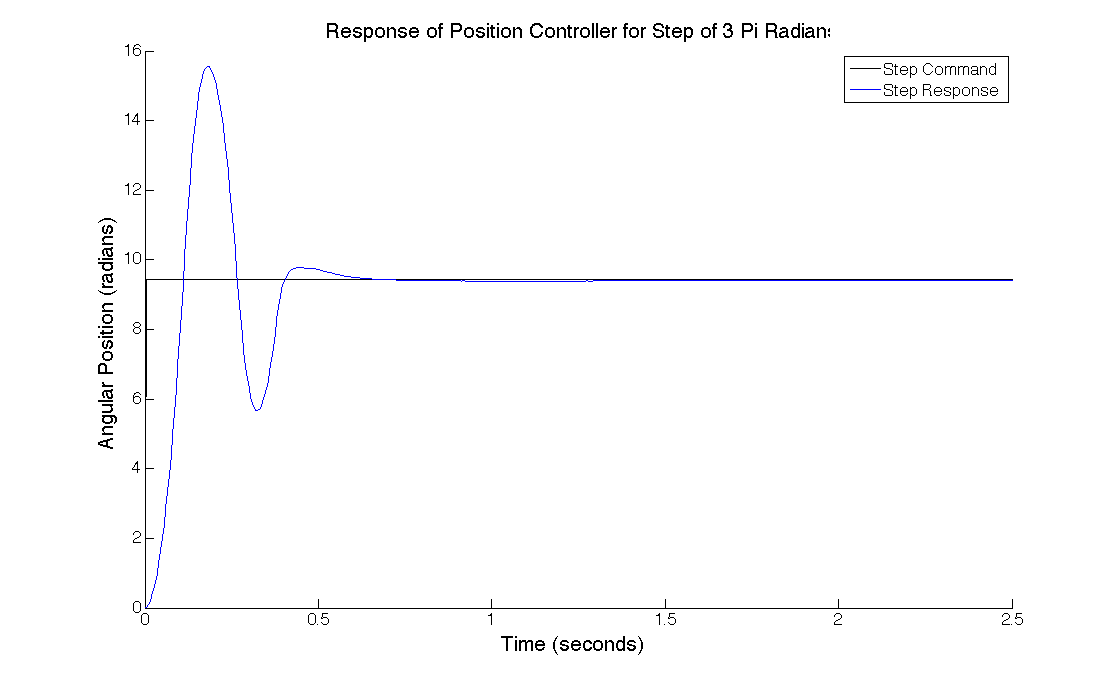
\includegraphics[width = 14cm]{posstep_3pi.png}
\caption{Step response of position controller}
\label{q5_b4}
\end{center}
\end{figure}

\begin{figure}
\begin{center}
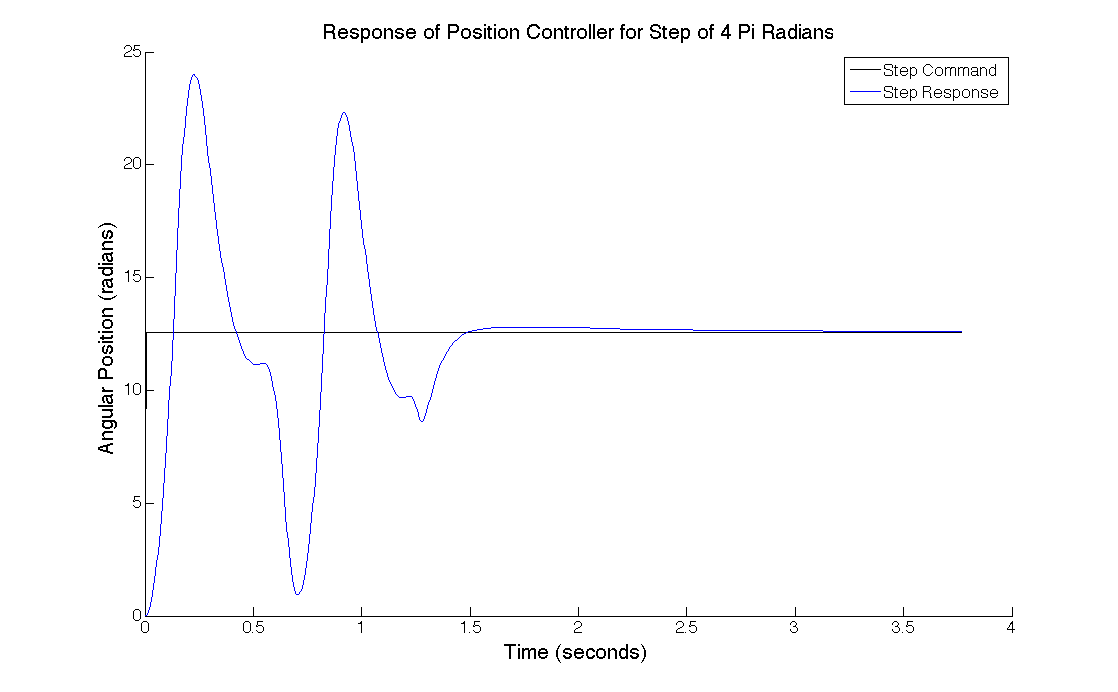
\includegraphics[width = 14cm]{posstep_4pi.png}
\caption{Step response of position controller}
\label{q5_b5}
\end{center}
\end{figure}

\subsection*{c. Quantization}

\section*{6.}

\begin{table}
\begin{center}
    \begin{tabular}{|c|c|c|c|c|c|c|}
        \hline
        Step Input Amplitude (Radians) & $0.5 \cdot \pi$ & $1 \cdot \pi$ & $1.5 \cdot \pi$ & $2 \cdot \pi$ & $5 \cdot \pi$ & $10 \cdot \pi$ \\ \hline
        Rise Time (seconds)            & 0.11            & 0.115         & 0.125           & 0.14          & 0.23          & 0.385          \\ 
        Settling Time (seconds)        & 1.5700          &1.6700          & 1.95500           & 1.9700        & 2.3050        & 2.8550         \\ 
        Percent Overshoot (\%)         & 4.3415          & 6.1564        & 7.9919          & 11.3925       & 21.091        & 27.1553        \\ 
        Steady State Error (\%)        & 0.11779         & 0.041862      & 0.053597        & 0.058333      & 0.050267      & 0.050634       \\
        \hline
    \end{tabular}
\end{center}
\end{table}

\begin{table}
\begin{center}
    \begin{tabular}{|c|c|c|}
        \hline
        Step Input Amplitude (Radians) & $2 \cdot \pi$ & $2 \cdot \pi$ with Noise \\ \hline
        Rise Time (seconds)            & 0.14          & 0.135                    \\ 
        Settling Time (seconds)        & 1.9700        &  -                    \\ 
        Percent Overshoot (\%)         & 11.3925       & 29.6000                  \\ 
        Steady State Error (\%)        & 0.058328      & 0.054649                 \\
        \hline
    \end{tabular}
\end{center}
\end{table}

\begin{figure}
\begin{center}
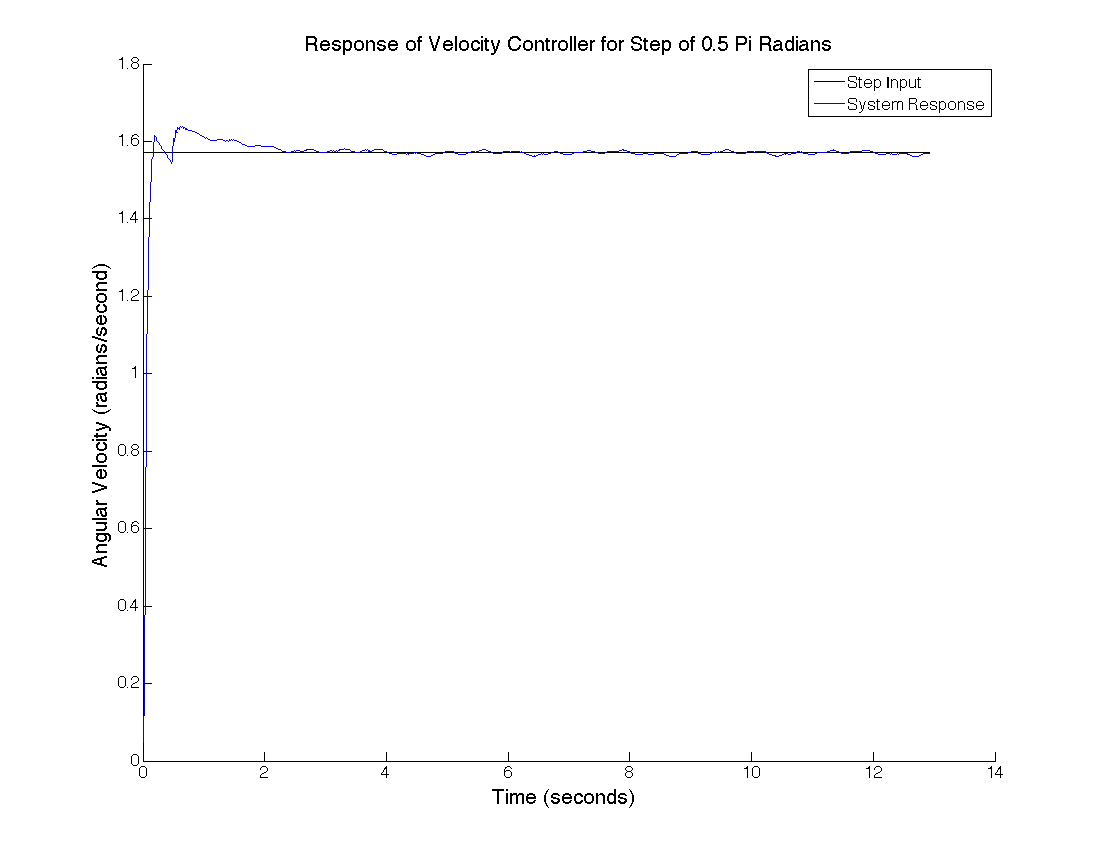
\includegraphics[width = 12cm]{velstep0_5Pi.png}
\caption{Velocity Controller Step Response}
\label{q6_1}
\end{center}
\end{figure}

\begin{figure}
\begin{center}
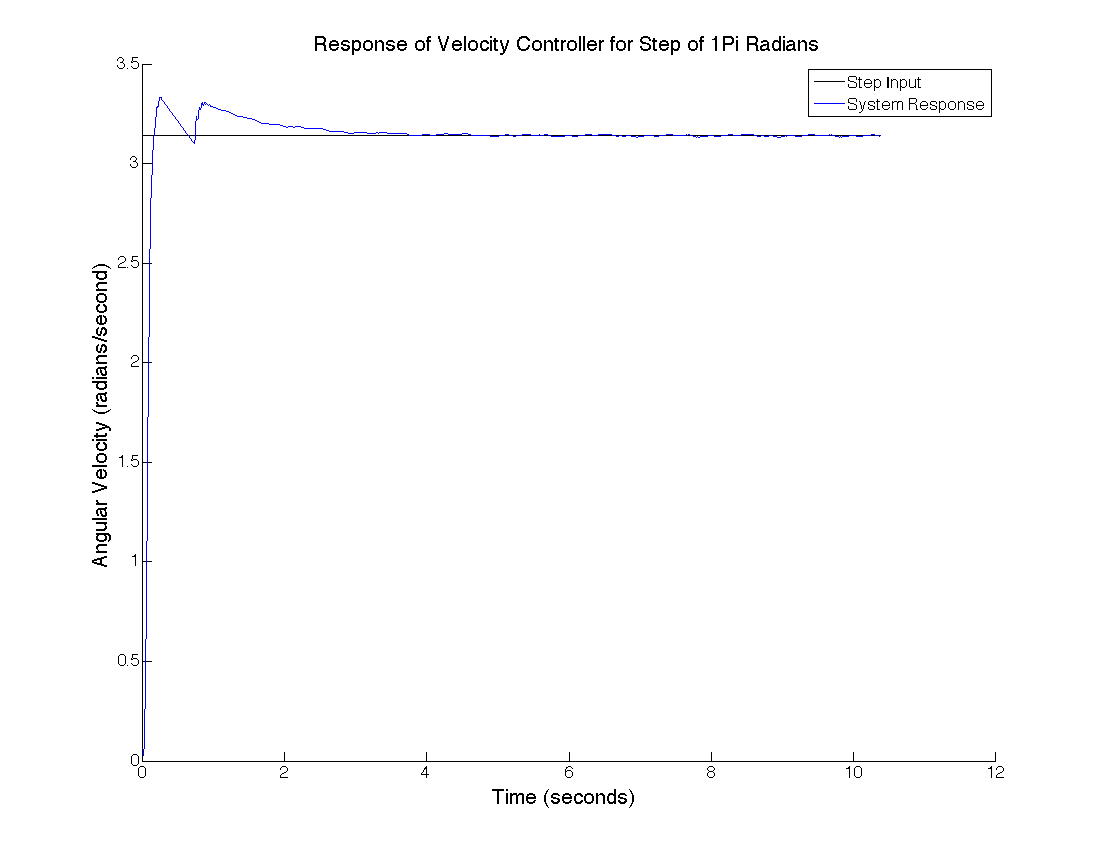
\includegraphics[width = 12cm]{velstepPi.png}
\caption{Velocity Controller Step Response}
\label{q6_2}
\end{center}
\end{figure}

\begin{figure}
\begin{center}
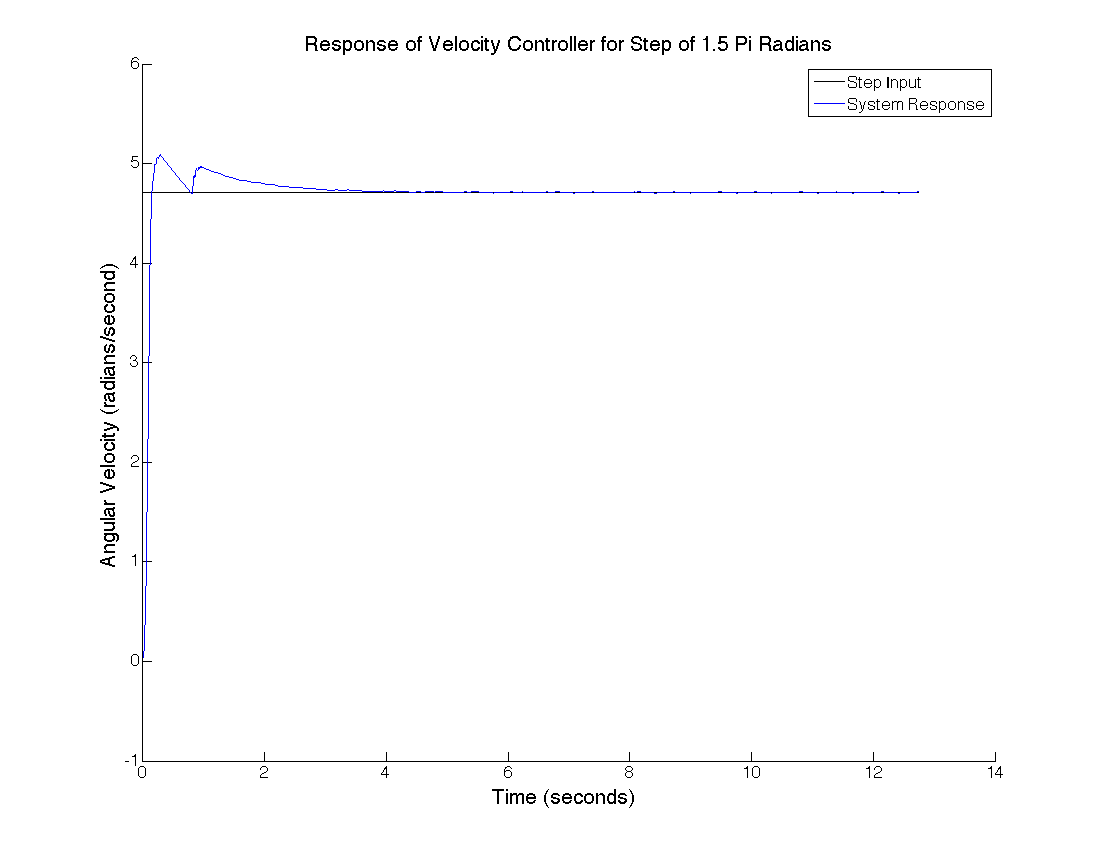
\includegraphics[width = 12cm]{velstep1_5Pi.png}
\caption{Velocity Controller Step Response}
\label{q6_3}
\end{center}
\end{figure}

\begin{figure}
\begin{center}
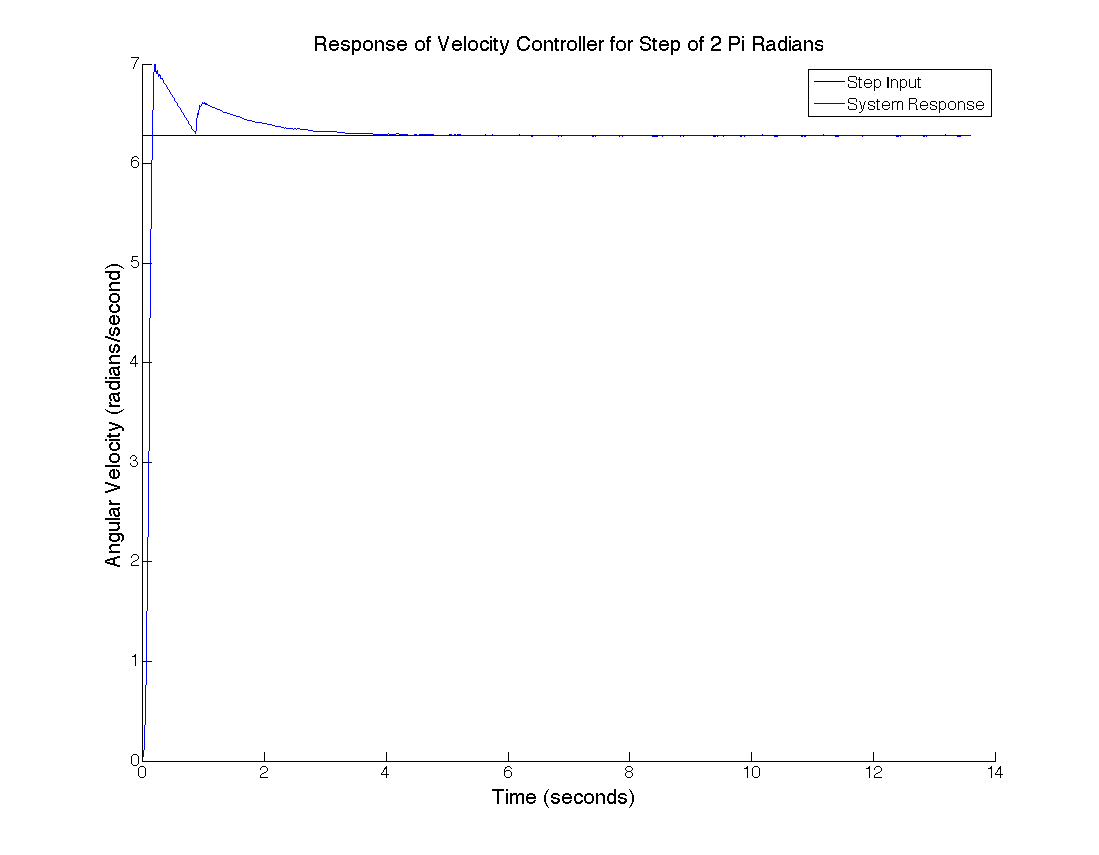
\includegraphics[width = 12cm]{velstep2Pi.png}
\caption{Velocity Controller Step Response}
\label{q6_4}
\end{center}
\end{figure}

\begin{figure}
\begin{center}
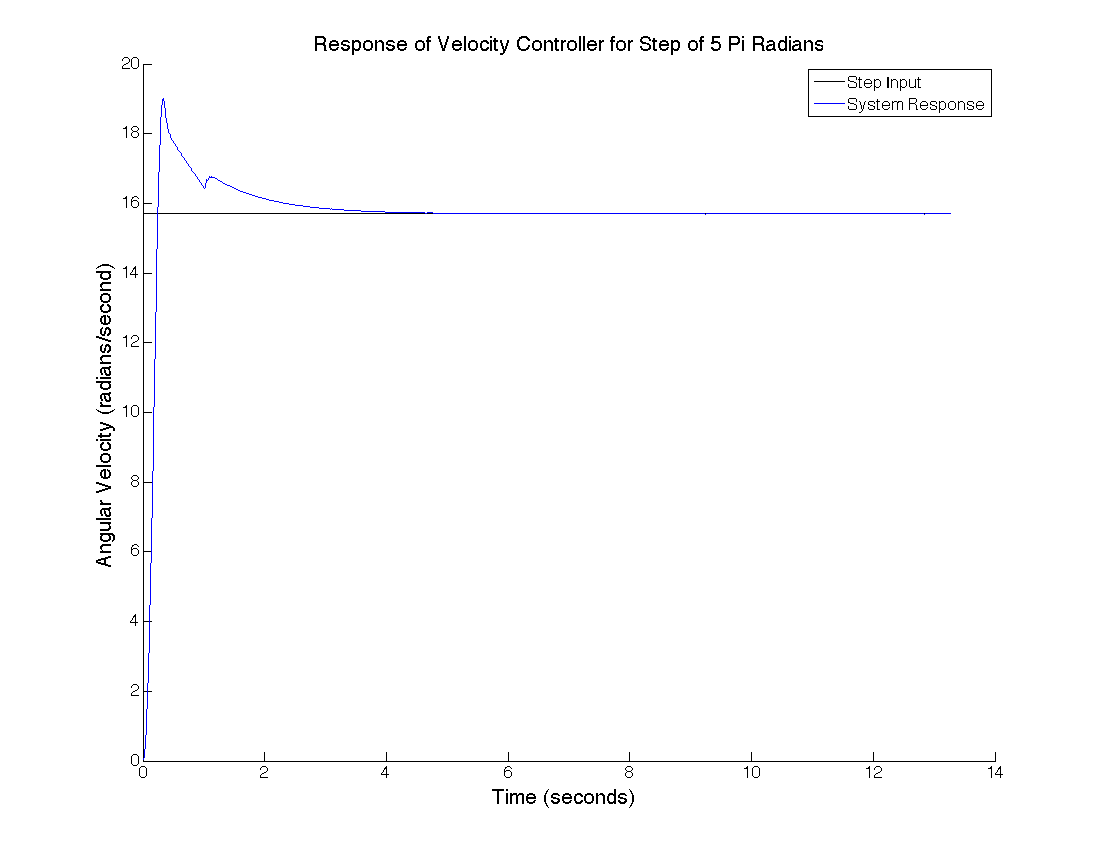
\includegraphics[width = 12cm]{velstep5Pi.png}
\caption{Velocity Controller Step Response}
\label{q6_5}
\end{center}
\end{figure}

\begin{figure}
\begin{center}
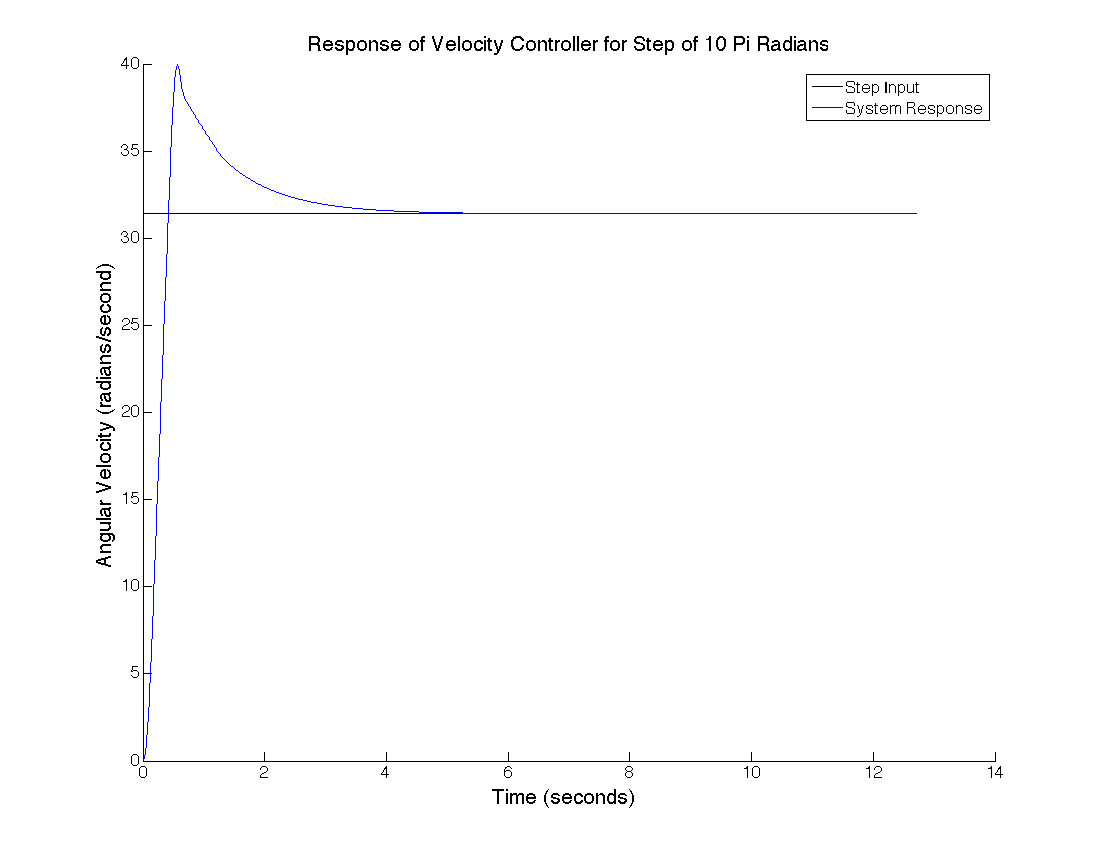
\includegraphics[width = 12cm]{velstep10Pi.png}
\caption{Velocity Controller Step Response}
\label{q6_6}
\end{center}
\end{figure}

\begin{figure}
\begin{center}
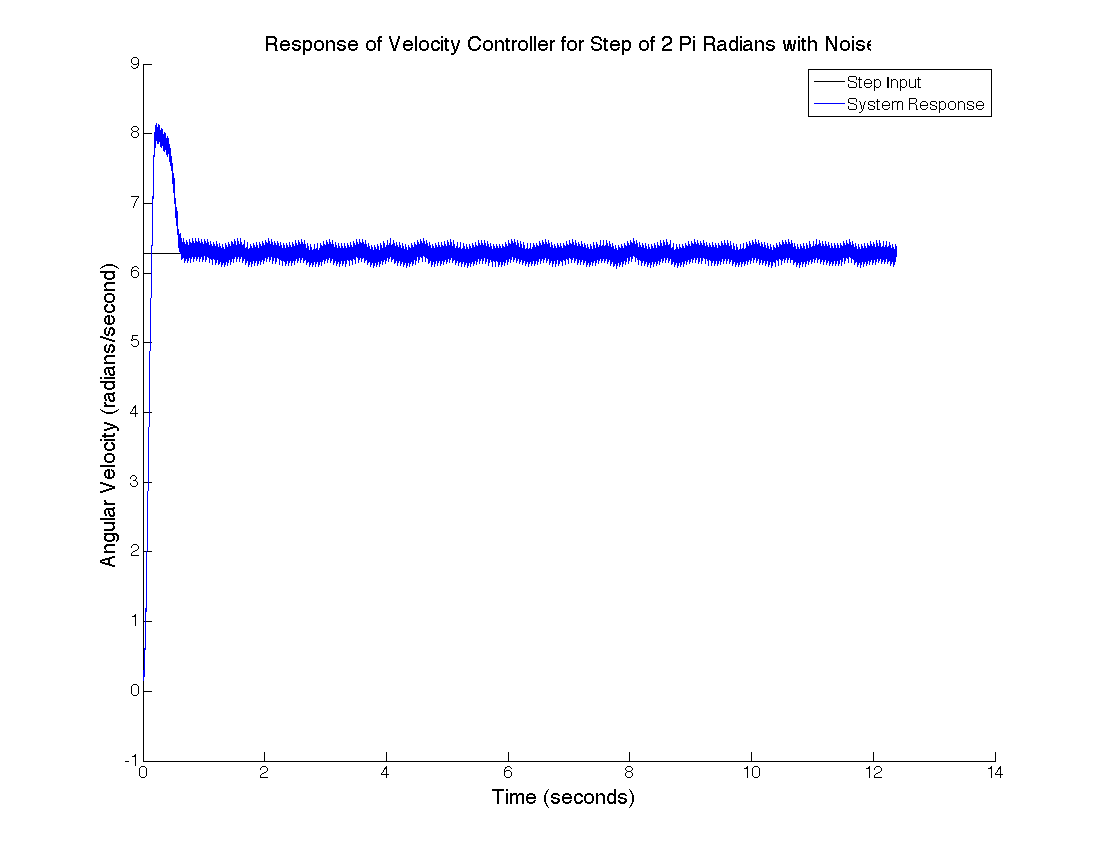
\includegraphics[width = 12cm]{velstep2PiwNoise.png}
\caption{Velocity Controller Step Response with added Noise}
\label{q6_7}
\end{center}
\end{figure}

\end{document}